\chapter{Tezos-specific Offline Design}\label{chap:offline_tezos}
After parsing an assertion contract and transforming it, the resulting AST is passed to the target-specific backend. For this thesis, the platform target is Tezos, with Michelson as the compilation target. This chapter continues to describe the pipeline stages implemented in the Tezos backend, which are shown in \figref{fig:pipeline_backend}. Furthermore, it states the necessary extensions to Michelson and its evaluator to facilitate useful assertions using random generators and assesses several orchestration strategies between the parent and assertion contract code. As a preliminary, the following section gives a short introduction to the Tezos blockchain, the Michelson language and some relevant tools in Tezos' ecosystem.

\section{Introduction to Tezos}\label{sec:tezos}
The Tezos blockchain is presented in its whitepaper as a \enquote{generic and self-amending crypto-ledger} \cite{goodman_tezos_2014}. It uses a proof-of-stake consensus mechanism that is not only used to agree on the current state of its ledger, but also allows its stakeholders to come to a consensus about changes in the economic protocol by participating in a voting process. The changes included in a protocol upgrade, called amendment, can influence i.a. which transactions are valid on the blockchain, the payment system or even the voting process itself without risking a fork of the blockchain. Everyone owning the cryptocurrency of Tezos, called Tez, is considered a stakeholder and can participate in the consensus mechanism. The whitepaper compares the self-amending protocol of Tezos to a game created by Philosopher Peter Suber called ``Nomic'', whose set of rules are subjected to a democratic voting system \cite{nomic}. Similar concepts can also be found in modern pop culture, such as the virtual sports league ``Blaseball'' \cite{blaseball} that became popular during the COVID-19 pandemic.

In addition to user accounts associated with a public key, Tezos supports smart contracts, which are written in the built-in language Michelson. Tezos' transaction fee system is similar to that of Ethereum \cite{wood_ethereum_2021} - it is gas-instrumented and besides a base fee, every operation and byte of storage during contract execution has to be paid for. However, Tezos imposes a hard cap on the amount of gas that can be consumed per operation (including internal transactions) \cite{tezos_docs}\cite{morley_repo}, whereas Ethereum limits the gas quota only in respect to blocks \cite{wood_ethereum_2021}.\\
Tezos is written in the multi-paradigm programming language OCaml \cite{ocaml_doc}. Compiling the its source code yields five essential binaries: the node, baker, endorser, accuser and client. The node is the entity that connects to the peer-to-peer network and keeps a copy of the chain. Bakers are responsible for producing new blocks, the endorsers for validating new blocks and the accusers to call out bakers or endorsers which double-sign or -endorse. The client provides a command line interface to interact with the local node through remote procedure calls (RPC).

\subsection{Proof-of-stake in Tezos}
In Tezos, contracts that staked a minimum amount of tokens, called a roll, can participate in the consensus mechanism and can either have the role of a baker or endorser. Contracts who don't own enough tokens or infrastructure to participate directly can delegate their baking and endorsing rights to other contracts. The rights are determined and assigned at the beginning of each cycle, which consists of a specified number of blocks. For baking, a random roll is selected for each block level and the rights are assigned to its owner. The block produced by that baker is endorsed by a fixed number of endorsers (currently 32 in protocol 008 Edo), which also have been assigned endorsing rights for this block level by a random selection of rolls. Since participants can stake more than one roll, an endorser may be assigned several endorsement slots at the same block level. \\
As an incentive for active participation in the consensus algorithm, delegates (and also delegators) receive rewards in form of tokens. However, if accusers detect double-baking or -endorsement, the delegate is penalized by burning (i.e., destroying) their security deposit. \cite{tezos_docs}

\subsection{Michelson}
Michelson is a lower-level, stack-based language with strict type-checking and supports primitive data types, like integers or strings, as well as high-level data structures such as list, maps and sum types \cite{tezos_docs}. The type system reduces the occurrence of runtime errors and ensures that only well-typed contracts are originated on the blockchain. \\
The concrete syntax of Michelson is called Micheline. A program is represented in Micheline nodes, which can be one of the following constructs:
\begin{itemize}
\item A constant of type integer (in decimal notation)
\item A constant of type string
\item A byte sequence in hexadecimal notation
\item An application of a language primitive to a sequence of nodes
\item A sequence of nodes
\end{itemize}
For documentation, readability and additional type constraints, Michelson and Micheline also offer three types of annotations - type, variable and field or constructor annotations, which are labelled with a unique special character in Micheline. The toplevel structure of a smart contract consists of a sequence of the three primitives \texttt{parameter, storage} and \texttt{code}, declaring the type of the input parameter, the storage type and the actual program code. The full grammar of Micheline and Michelson can be found in the Tezos developer resources \cite{tezos_docs}.

\subsubsection{Entrypoints}
Unlike the contracts shown so far, which were expressed with the syntax of Ethereum's contract language Solidity \cite{solidity_docs}, Michelson doesn't have a concept of named functions with individual input parameter types. Instead of named functions, Michelson programs can have separate entrypoints by taking a disjunctive type as input parameter and optionally tagging the type constructors with a "function" name. The disjunctive type is built by nesting the \texttt{or} type, which has the constructors \texttt{left} and \texttt{right}. Assume we want to implement the contract from \lstref{lst:prime} in Michelson and add another function to it, which expects a string parameter. Omitting the actual program, the contract type declaration looks as follows:
\begin{lstlisting}[language=Michelson, numbers=none, caption=Michelson contract with two entrypoints, label=lst:entrypoints]
parameter (or (int %isPrime) (string %isUpper));
storage unit;
code {
  ...
  IF_LEFT { ... (* then *)}
          { ... (* else *)}
}
\end{lstlisting}
The input type declared in the primitive application \texttt{parameter} accepts input of either type \texttt{left int}, or \texttt{right string}. By adding the field annotations \texttt{isPrime} and \texttt{isUpper}, the entrypoints are given tags and can be called explicitly by an external transaction. In that case, parameters of type \texttt{int} or \texttt{string} are accepted and the value is automatically wrapped into the respective constructors. Furthermore, it's possible to declare a \texttt{default} entrypoint, which is called when no explicit tag is specified. By default, the default entrypoint is assigned to the root of the parameter type. \cite{tezos_docs}

\subsubsection{Internal operations}
Smart contracts are able to call other smart contracts by emitting internal operations. The return type of Michelson programs is a tuple of a list of internal operations and the updated storage. Thus, after the actual contract has been executed, the operations of the returned list are run in sequence. Since the internal operations may in turn also emit internal operations, they are put into a queue and are processed in order. As an example, \figref{fig:internal_ops} shows an execution order of two external transactions in sequence, i.e., transactions which have been initiated by a user account, and their internal operations.
\begin{figure}[h]
\centering
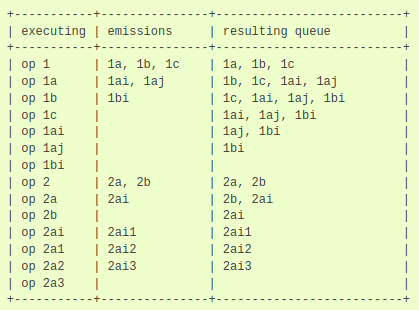
\includegraphics[width=0.5\linewidth]{figures/4-offline_tezos/internal_ops}
\captionsource{Execution order of two external operations and their internal operations}{\cite{tezos_docs}}
\label{fig:internal_ops}
\end{figure}

Both external and internal operations can fail if the source does not have enough balance to spend the specified amount, a gas limit was reached or if a program fails when reaching a \texttt{FAILWITH} instruction. If a failure occurs, the whole sequence fails and all changes up to the point of failure are reverted.

\subsection{Gas model}
In Tezos data is stored and transmitted as byte sequences --- in order to obtain a typed representation of their value for interpretation, a byte sequence is first deserialised into Micheline and subsequently parsed \cite{tezos_repo}. Conversely, before transmitting or storing something on the blockchain, the typed representation is first unparsed and then serialised. The gas consumption of an operation, e.g. a transaction or an origination, is thus composed of the following positions on top of a base cost \cite{morley_gasmodel}\cite{tezos_repo}:
\begin{enumerate}
\item \textbf{Reading costs} --- apply for reading contract code, storage or Big Maps from the internal database and, on top of the base cost, depend on the amount of bytes read
\item \textbf{Deserialization costs} --- depend on the Micheline expression and their size
\item \textbf{Parsing costs} --- are composed of three types of parsing costs:
	\begin{itemize}
	\item type parsing --- apply when a Micheline node is converted into a valid type and are computed by a recursive formula; parametrized types therefore generate more cost than plain types
	\item data parsing --- apply when a node is converted into the value of a known type and depend on the byte length for non-parametrized types, on the number of contained elements for container types and on the parameters for parametrized types
	\item code parsing --- computes the return type of the code by sequentially applying instructions and type checking if the result matches the expectation.The cost thus increases in the number of instructions, while some instructions incur additional costs besides their base cost, such as \texttt{IF} (both branched need to be checked and compared) or \texttt{CREATE\_CONTRACT} (called contracts needs to be type checked)
	\end{itemize}
\item \textbf{Type comparison costs} --- occur during parsing when types are checked for equality (e.g. when verifying that the branches of \texttt{IF} have the same type) or contract execution
\item \textbf{Interpreter costs} --- apply for each executed instruction and are specified for each. Expensive instruction are, for instance, \texttt{CONTRACT} with a high base cost and additional cost for reading, deserializing and type checking of the target contract code. 
\item \textbf{Unparsing costs} --- depend on the type of the data; parametrized types incur cost for unparsing its inner types as well
\item \textbf{Serialization costs} --- depend, similar to deserialization, on the Micheline expression and their size
\item \textbf{Writing costs} --- apply when writing to the internal database. Depend on the amount of bytes written, but with a higher base cost than reading. Additional cost is inflicted if the storage of the contract increased in size
\end{enumerate}
If a transaction emits internal operations, their gas consumption is computed in the same way and are added to the total gas consumption of the external operation.

\subsection{Developer tools in the Tezos ecosystem}
This section describes some relevant tools and projects for developers that are part of Tezos' ecosystem.

\subsubsection{Tezos Libraries}
Tezos' executables and libraries are developed in the programming language OCaml and are available on through OCaml's package manager \texttt{opam} \cite{tezos_opam}. The protocol libraries of every version are released separately, thus any projects can be built on the protocol of choice. Important libraries that were used in the development of the offline toolchain are the Micheline library providing the internal abstract syntax tree (AST) and parser of the Michelson language, as well as the protocol specific libraries containing i.a. the type checker. Additionally, the client libraries are used to retrieve any needed information from the node or blockchain via RPCs.

\subsubsection{Testing tools}
Before a new protocol is proposed to the Tezos network, it has to be thoroughly tested with system, integration and regression tests. This requires a sandboxed network to simulate the real peer-to-peer network, such that also interactions between the actors of the blockchain can be tested. Tezos' development environment provides two testing frameworks for this:
\begin{itemize}
\item[\textbf{Flextesa}] With Flextesa (Flexible network sandboxes)\cite{tezos_docs} one can configure and run a small, fully functional sandboxed test network including nodes, bakers, endorsers and accusers. Accounts can be instantiated and used to send or receive funds. Configurable are, for instance, the size of the network, the time between blocks or enabling generation of random network traffic. Networks may either be fully autonomous, baking blocks automatically, or require manual baking of blocks. It also supports interactive sessions, where the tester can interact with the blockchain using the Tezos client. Flextesa's typical use-cases are interactive testing scenarios like double-baking, the voting process or protocol amendments. The Tezos repository already provides ready-to-use scenarios for accusations. Besides testing shell or protocol code, Flextesa can also be used to test smart contracts.
\item[\textbf{Tezt}] The Tezt framework \cite{tezos_docs} is newer than Flextesa and planned as its replacement. It launches the Tezos binaries as external processes to build a sandboxed test network of configurable size. Its main advantages over Flextesa are simplicity, better usability and extendibility and better performance due to the use of an event system instead of polling the node.
\end{itemize}

\subsubsection{High-level languages}
Michelson is a compilation target for various high-level languages that provide a more user-friendly and intuitive way of writing smart contracts. Additionally, some of them come with development environments and testing or verification tools. The following list comprises of the three most prominent languages that compile to Michelson:
\begin{itemize}
\item[\textbf{Liquidity}] \cite{liquidity} is a language with an OCaml-like syntax, which allows using local variables instead of stack manipulations. Its module system can be used to write reusable contract code or libraries. Besides an optimizing compiler, the project also includes a decompiler to compile Michelson programs to Liquidity.
\item[\textbf{SmartPy}] \cite{smartpy} is a language available through a Python library and lets developers write contracts and tests using Python syntax and structures (such as classes). Its developer suite includes i.a. a compiler, a simulation engine for testing contracts and an online editor.
\item [\textbf{Ligo}] \cite{ligo} offers multiple syntax flavours that are close to Pascal, OCaml or Reason. Besides compilation, the toolchain allows to invoke or evaluate the generated code locally. The Ligo OCaml packages can be integrated into other OCaml projects, s.t. the compiler can be invoked from within third-party applications.
\end{itemize}

\section{Extensions to Michelson}
The way Michelson is interpreted is purely functional; it takes the current stack and an operation and builds a return stack from the initial one, without causing any side effects \cite{tezos_docs}. The recursive Michelson interpreter is defined as as a list of rules comprising of all possible inputs, i.e. program and stack types, and the respective output stack type of the computation if a rule applies. Each rule is of the following form: 
\begin{lstlisting}[caption=Rules form in the Michelson interpreter \cite{tezos_docs}, language=, numbers=none, label=lst:rules]
> (syntax pattern) / (initial stack pattern)  =>  (result stack pattern)
    iff (conditions)
    where (recursions)
    and (more recursions)
\end{lstlisting}
For each valid program and initial stack exactly one rule matches (given that any extra conditions over values on the stack, stated after the \texttt{iff} keyword are true) \cite{tezos_docs}. If the result depends on the results of other program interpretations (given after the keywords \texttt{iff, where, and} in rule form), the rule only applies if these partial results also match the respective intermediate result stack patterns.\\
In addition, there exists a typing rule for each syntax construct that restricts the valid input stacks. The typing rules use the meta variables \texttt{'a} for type and \texttt{'A} for stack type variables in order to express consistency within the program (not polymorphism). These rules are given in the following form:
\begin{lstlisting}[caption=Form of typing rules in Michelson's specification \cite{tezos_docs}, language=, numbers=none, label=lst:type_rules]
(syntax pattern)
:: (type of stack before) -> (type of stack after) [rule-name]
   iff (premises)
\end{lstlisting}
The type notations, as well as syntax and stack patterns are listed in \cite{tezos_docs}.

Since Michelson is implemented in the protocol-specific part of the blockchain code, adding new instructions require a protocol update. The instruction must be added i.a. to the list of tokens, its computation to the interpreter and its typing rules to the type checker. As the computation of the new instruction must be paid for like any other instruction, the protocol must also specify a gas cost. Previous extensions to the Michelson language, such as \cite{tezos_michelson_ext}, can be used as a guideline for the implementation and the gas cost specification in \cite{tezos_repo_gas} as an orientation to how high the gas costs should be scheduled for comparable instructions.

From the given formulas and assertion examples so far, one can derive a set of necessary instructions that need be be present in the target language. The following subsections list the instructions which have to be added to Michelson's instruction set, specify their selection and typing rules and describe how they can be implemented in the interpreter. These do not necessarily include high level instructions, like \texttt{sqrt} from \eqref{eq:prime}, that can be reproduced by using lower level instructions. For these purposes, a later iteration of the syntax will provide the feature of user-defined functions.

\subsection{random}
A vital instruction that cannot be expressed with Michelson's current instruction set (state of protocol 008 Edo \cite{tezos_docs}) is the generation of a random value of certain types. Since smart contracts need to be deterministic, s.t. the network can reach a consensus about the state of the ledger \cite{chatterjee_probabilistic_2019}, the prevalent workarounds for generating pseudo-random numbers cannot be used for assertion checking. Distributed assertion checking explicitly requires as many validators as possible to generate a unique value, whereas common schemes for randomness, like oracles or using block attributes as seeds \cite{chatterjee_probabilistic_2019}, will provide the same values for all validators.\\
\lstref{lst:rand_type} specifies the selection and typing rule of a new instruction \texttt{rand}, which consumes an offset and a positive range from the stack and pushes a randomly generated integer to the top. This instruction, of course, can also be provided for other data types, such as \texttt{nat}, \texttt{string} or \texttt{mutez}.
\lstset{upquote=true}
\begin{lstlisting}[caption=Selection and typing rules of the integer \texttt{rand} instruction, language=, numbers=none, label=lst:rand_type]
:: int : nat: 'A -> int : 'A
> RAND/ offset : range : S  => int : S
\end{lstlisting}

Within the Michelson interpreter, the selection of rules is implemented as a huge match case \cite{tezos_repo}. If the rule for \texttt{rand} applies, the respective computation in OCaml could look as drafted in \lstref{lst:rand_impl}.
\begin{lstlisting}[caption=Simplified evaluation of \texttt{rand} in the Michelson interpreter, language=, label=lst:rand_impl]
match (instruction, stack) with
...
| (Rand (offset, (range, rest))) -> 
   Random.self_init;
   let rand_int = offset + Random.int(range) in
   return (rand_int, rest)  (* Resulting stack *)
\end{lstlisting}

\subsection{nth}
An exception for not adding higher level instructions may be the more fundamental operation \texttt{nth} for accessing list elements, as it is used (sometimes more than once, ref. \eqref{eq:sorted_v2}) in many use cases. Adding an own predefined primitive for this reduces the origination costs of the assertion contract, given that its equivalent in the current instruction set requires the compiler to generate a workaround using iteration, for instance a loop or list iterator. As a first approximation, appendix \ref{apx:nth} shows a potential implementation of \texttt{nth} in Liquidity (\lstref{lst:nth_liq}) using a loop, and how the respective Michelson code looks like after compiling the contract with the Liquidity compiler (\lstref{lst:nth_tz}). \\
In case the \texttt{nth} is added as a predefined primitive to Michelson for the type \texttt{'a list}, its selection and typing rules are specified as follows:
\begin{lstlisting}[caption=Selection and type rule of the list \texttt{nth} instruction, language=, label=lst:nth_type]
:: (list 'a) : nat : 'A -> option 'a : 'A
> NTH / l : index : S  =>  Some 'a: S
     iff index is within bounds
> NTH / l : index : S  =>  None 'a: S
     iff index is out of  bounds
\end{lstlisting}
As Michelson lists are represented with OCamls list type within the VM \cite{tezos_repo}, the computation for \texttt{nth} could look as shown in \lstref{lst:nth_impl}.
\begin{lstlisting}[caption=Simplified evaluation of \texttt{nth} in the Michelson interpreter, language=, label=lst:nth_impl]
match (instruction, stack) with
...
| (Nth ({elements = []; _}, (_, rest))) ->
  return ((None, rest)
| (Nth ({elements = es; length}, (index, rest))) ->
  let l_length = of_int length in
  if index <= l_length
    then return (Some (List.nth es index), rest)
    else return (None, rest)
\end{lstlisting}
\lstset{upquote=false}

\section{Orchestration of contract and assertions}
So far, the assertion and parent contract have been considered separately. However, on the blockchain they have to be orchestrated, s.t. the bakers and validators execute the assertion before the actual contract code. The orchestration does not only include the linking of assertion and contract code, but also a mechanism to execute an assertion $t$ times depending on the domain space that needs to be checked. There are basically two approaches - the assertion and contract code can be assembled into a single monolithic contract, or they can be originated separately as standalone contracts. As the strategy has an impact on the compilation process and output, it has to be determined in advance which of the two should be implemented and how.

\subsection{Approach 1: Monolithic contract}
In the monolithic approach, a new contract is built using both the assertion and parent code as input. As is outlined in \figref{fig:monolithic_orchestration_basic}, the assertions can either be appended to the original contract as separate entrypoints or by prepending them to the code of the respective entrypoint. This tightly couples and unites the code in one self-contained unit.
\begin{figure}[!htb]
\subfloat[Appending assertions as separate entrypoints]{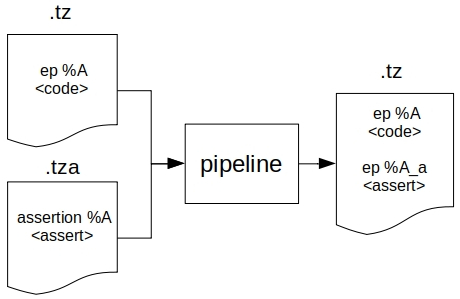
\includegraphics[width=0.5\textwidth]{figures/4-offline_tezos/pipeline_output_mono_ep_basic.jpg}}
\quad
\subfloat[Inserting the assertion code into the original entrypoint]{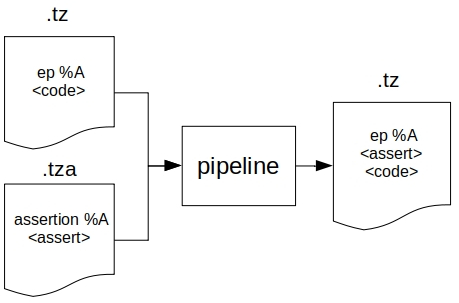
\includegraphics[width=0.5\textwidth]{figures/4-offline_tezos/pipeline_output_mono_basic.jpg}}
\caption{Approaches for assembling a monolithic contract}
\label{fig:monolithic_orchestration_basic}
\end{figure}
While the link between assertion and contract code is already given in a), the entrypoint and assertions in b) still need to be coupled, as it is not inherent which entrypoint represents a normal and which the respective assertion. For this reason, assertion entrypoints need to have fixed name pattern, s.t. it is derivable from the original entrypoint. As a proposal, the tag of the assertion is the tag of its parent entrypoint suffixed with a \texttt{\_a}, e.g. \texttt{A\_a} for entrypoint \texttt{A}. The baker can then execute the contract normally by calling the original entrypoint and prompt the validators to execute the assertion separately. \\
Both approaches, however, do not yet provide any means to have validators execute the assertions $t$ times. Since only the contract itself knows how to calculate $t$ (as per the range(s) of the random generator(s)), it cannot be passed to the validators as a parameter to the validation request. Instead, the contract itself needs a test run manager which handles this. A test run manager can either be implemented as another entrypoint, say \texttt{A\_m}, which then calls \texttt{A\_a} (or \texttt{A} in case of a)) $t$ times as an internal operation. Because transactions on Tezos guarantee either total success or total failure \cite{tezos_docs}, the execution is stopped as soon as one of the internal operation fails, i.e. detects a counterexample. When extending the diagram for a) with the manager, the pipeline output thus look as shown in \figref{fig:monolithic_orchestration}. The output for b) is analogue.
\begin{figure}[h]
\centering
  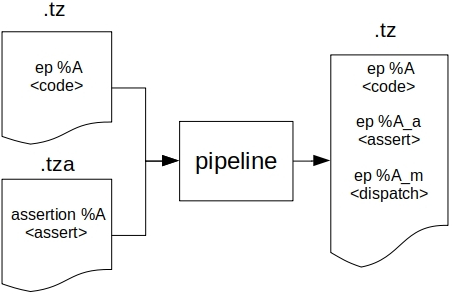
\includegraphics[width=0.5\textwidth]{figures/4-offline_tezos/pipeline_output_mono_ep.jpg}
	\caption{Monolithic assembly with separate entrypoints for manager and assertion}
	\label{fig:monolithic_orchestration}
\end{figure}
Another possibility is to create a separate manager contract that acts as a proxy, contains the manager code and internally calls the monolithic contract. This solution is a hybrid of the monolithic and modular approach. The section covering the modular approach describes in more detail how it is implemented.\\
It's important to realize that neither baker nor validators can differentiate between entrypoints that have an associated assertion and those that do not. In order to avoid transaction failures caused by calling assertions that do not exist, the compiler has to add dummy managers for empty assertions that call the actual contract code immediately. \lstref{lst:manager} drafts the manager code for entrypoints with and without assertions in pseudocode (assuming a purely monolithic implementation). 
\begin{lstlisting}[label=lst:manager, caption=Implementation of the manager in pseudocode]
%A (i : int) { ... }

%A_a (i : int) { .. assert (...) }

%A_m (i : int) {
	n = compute_n(i)
	Do m = 1 to n
		call(self, A_a, i)
}

%B (j : int) { ... }

%B_m (j : int) { call(self, B, j) }
\end{lstlisting}

\figref{fig:interaction_monolithic} and \ref{fig:interaction_monolithic_managertz} depict the interaction of the baker and validators with the resulting contracts on the blockchain for a variant using a single monolithic contract versus a hybrid solution. After calling a contract that includes an assertion, the baker has to keep the transaction in its mempool, a buffer where a node keeps prevalidated transactions not yet included in a block \todo{remove explanation if added to Tezos chapter}. Before it can be included, the transaction has to be kept there for a minimum amount of time, s.t. the validators have enough time to validate the assertion \todo{refer to blockchain protocol chapter if there is one}. The bakers therefore need to execute such transactions in a dedicated ``challenge'' mode, which could be signalled by using a special operation type to call such contracts. Operation types in Tezos are, i.a., transactions, originations or endorsements. By adding, for instance, a special transaction type (abbreviated by \texttt{txa} in the interaction diagrams), bakers can differentiate between normal transactions and those with assertions.
\begin{figure}[h]
\centering
  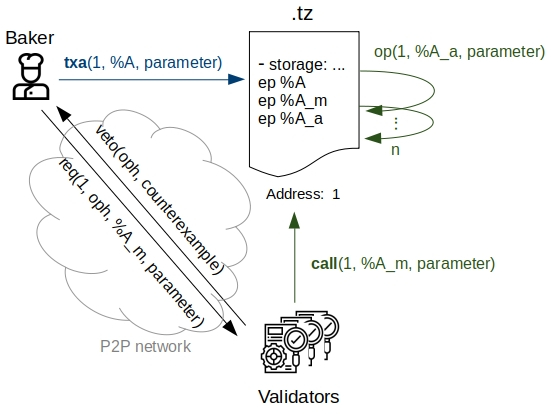
\includegraphics[width=0.7\textwidth]{figures/4-offline_tezos/interaction_monolithic.jpg}
	\caption{Interaction with a monolithic contract}
	\label{fig:interaction_monolithic}
\end{figure}

\begin{figure}[h]
\centering
  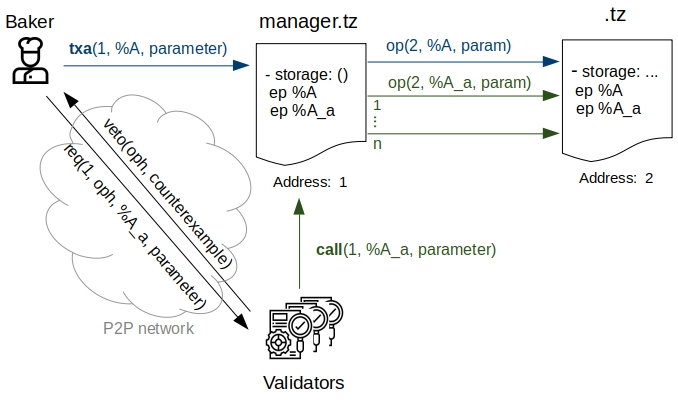
\includegraphics[width=0.8\textwidth]{figures/4-offline_tezos/interaction_monolithic_managertz.jpg}
	\caption{Interaction with a manager and monolithic contract}
	\label{fig:interaction_monolithic_managertz}
\end{figure}

After prevalidating a transaction in the challenge mode, the baker then sends a request to the network to check the associated assertion. The request contains the address of the monolithic contract or manager, the operation hash (oph) of the prevalidated transaction, the derived entrypoint tag of the assertion and the parameter. The operation hash is used to relate a counterexample to the respective transaction. Upon receiving such a request, the validators call the assertion manager; what type of operation is used for is an open question for the protocol design. For efficiency, at most the test runs detecting a counterexample should be recorded on the blockchain, which would not be the case if validators use standard transactions. What has been left out so far in the offline design is the representation of a counterexample. \secref{} briefly discusses this as an open question and follow-up of this thesis \todo{secref}.

\subsubsection{Evaluation of the monolithic approach}
The presented implementations of the monolithic approach each have strengths and weaknesses. Generally, they all share a pivotal disadvantage - they require a modification of the parent contract. This not only complicates the compilation process by requiring a decompilation of the parent code and an interweaving of the assertion code, but it also restricts the integration of assertions to contracts that have not yet been originated on the blockchain. \lstref{lst:mono} shows the skeleton of a monolithic contract that results from the given parent and assertion contract; both the parameter type and the branching of the code body have to be adapted. Another problem are contract invocations using the default entrypoint: firstly, the derivation of the entrypoint for the assertion becomes considerably more complex, as no explicit tag is given. Secondly, the parameter cannot be passed unmodified to the assertion, because the parameter types in respect to the default entry point do not match. For instance, invoking the default entrypoint of \texttt{example\_monolithic.tz} (\lstref{lst:mono}) with parameter \texttt{Left 4} calls \texttt{A}, but the respective assertion \texttt{A\_a} expects the value as \texttt{Left (Left 4)}. \\
Due to the tight coupling of parent and assertion code, this approach is also inflexible, since adaptions to either part require a recompilation and new origination of the whole code.
\lstinputlisting[label=lst:mono, caption=Skeleton of a monolithic contract in Michelson, numbers=left]{listings/monolithic.tz}

The distinct advantages and disadvantages of each combination of given implementation approaches are described briefly in the following matrix in \tabref{tab:mono_eval}.
\begin{table}[h]
	\centering
	\newcommand{\tabitem}{~~\llap{\textbullet}~~}
	\caption{Advantages and disadvantages of monolithic implementations}
	\label{tab:mono_eval}
	\subfloat[Monolithic w/ manager and assertion entrypoints] {
		\centering
		\begin{tabular}{ | p{0.5\linewidth} | p{0.5\linewidth} |}
		\hline
		\thead{Advantages} & \thead{Disadvantages} \\ \hline
		\begin{itemize}[leftmargin=*,noitemsep,topsep=0pt,parsep=0pt,partopsep=0pt]
		\item Contract and assertion can be called separately $\rightarrow$ parent code is only executed once
		\end{itemize} &
		\begin{itemize}[leftmargin=*, noitemsep,topsep=0pt,parsep=0pt,partopsep=0pt]
		\item More complex compilation; adds 1-2 entrypoints per native entrypoint
		\item Less readability
		\end{itemize} \\ \hline
		\end{tabular}
	}

	\subfloat[Monolithic w/ manager entrypoints and prepended assertion] {
		\centering
		\begin{tabular}{ | p{0.5\linewidth} | p{0.5\linewidth} |}
		\hline
		\thead{Advantages} & \thead{Disadvantages} \\ \hline
		\begin{itemize}[leftmargin=*, noitemsep,topsep=0pt,parsep=0pt,partopsep=0pt]
		\item Bypassing the assertion is not possible
		\end{itemize} &
		\begin{itemize}[leftmargin=*, noitemsep,topsep=0pt,parsep=0pt,partopsep=0pt]
		\item Cost inefficient - validators execute the assertion + code $t$ times
		\item Also only works with explicit entrypoint tags
		\end{itemize} \\ \hline
		\end{tabular}
	}

	\subfloat[Hybrid w/ manager and assertion entrypoints] {
		\centering
		\begin{tabular}{ | p{0.5\linewidth} | p{0.5\linewidth} |}
		\hline
		\thead{Advantages} & \thead{Disadvantages} \\ \hline
		\begin{itemize}[leftmargin=*, noitemsep,topsep=0pt,parsep=0pt,partopsep=0pt]
		\item Contract and assertion can be called separately
		\item Modularity $\rightarrow$ manager contract can be adapted independently
		\item Readability
		\end{itemize} &
		\begin{itemize}[leftmargin=*, noitemsep,topsep=0pt,parsep=0pt,partopsep=0pt]
		\item Higher initial origination costs due to more boilerplate code
		\end{itemize} \\ \hline
		\end{tabular}
	}

	\subfloat[Hybrid w/ manager entrypoints and prepended assertion] {
		\centering
		\begin{tabular}{ | p{0.5\linewidth} | p{0.5\linewidth} |}
		\hline
		\thead{Advantages} & \thead{Disadvantages} \\ \hline
		\begin{itemize}[leftmargin=*, noitemsep,topsep=0pt,parsep=0pt,partopsep=0pt]
		\item Bypassing the assertion is not possible
		\item Modularity
		\item Readability
		\end{itemize} &
		\begin{itemize}[leftmargin=*, noitemsep,topsep=0pt,parsep=0pt,partopsep=0pt]
		\item Cost inefficient - validators execute the assertion + code $t$ times
		\item Higher initial origination costs due to more boilerplate code
		\end{itemize} \\ \hline
		\end{tabular}
	}
\end{table}

\subsection{Approach 2: Modular contracts}\label{sec:modular}
With the modular approach, the assertion manager and each of the assertions are originated as separate contracts on the blockchain. The manager mirrors the interface of the parent contract, while each assertion each only has a single entrypoint which expects the raw parameter type. Due to the ``outsourcing'' of the assertion code, the parent contract remains pure and does not have to be modified. Similar to the hybrid solution from the last section, the manager calls the respective assertion contract $t$ times as an internal operation before calling the actual contract. In the case of empty assertions, it calls the parent contract immediately. Correspondingly, the pipeline outputs 1-$m$ contracts, where $m$ is the amount of entrypoints with an associated assertion, as depicted in \figref{fig:modular_assembly}.
\begin{figure}[h]
\centering
  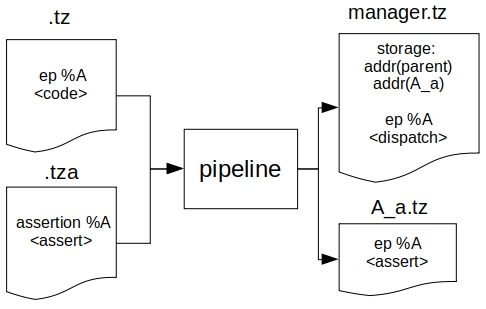
\includegraphics[width=0.6\textwidth]{figures/4-offline_tezos/pipeline_output_modular.jpg}
	\caption{Modular assembly of assertion and manager code}
	\label{fig:modular_assembly}
\end{figure}

In order to link the separate contracts to each other, the manager needs to know the addresses of the other contracts, which ultimately entails a fixed origination order. The independent assertion and parent contract(s) have been originated first, so that their addresses can be passed to the manager as initial storage values. If the storage is structured as a map from a unique identifier to an address, the entrypoints of the manager can then look up the address with its assigned identifier. The assignment of identifiers to entrypoints is hard-wired during the compilation, as is shown in the pseudocode for the manager contract in \lstref{lst:manager_modular}. The corresponding initial storage for the given contract is the mapping \texttt{{0: <addr parent>; 1: <addr A\_a>; 2: <addr B\_a}}.
\begin{lstlisting}[label=lst:manager_modular, caption=Implementation of the modular manager in pseudocode]
storage (map int address);

%A (i : int) {
	n = compute_n(i)
	Do m = 1 to n:
		call(storage.get(1), i)
	call(storage.get(0), A, i)
}

%B (j : int) {
	n = compute_n(j)
	Do m = 1 to n:
		call(storage.get(2), j)
	call(storage.get(0), B, j)
}
\end{lstlisting}

The interaction with the contracts in the modular approach is shown in \figref{fig:interaction_modular}. Even though the transactions shown in the diagram state an explicit entrypoint tag, contracts can, of course, also be called through \texttt{\%default}. In that case, the parameter passed with the internal operations to \texttt{A\_a.tz} is not equivalent, but the raw parameter value.
\begin{figure}[h]
\centering
  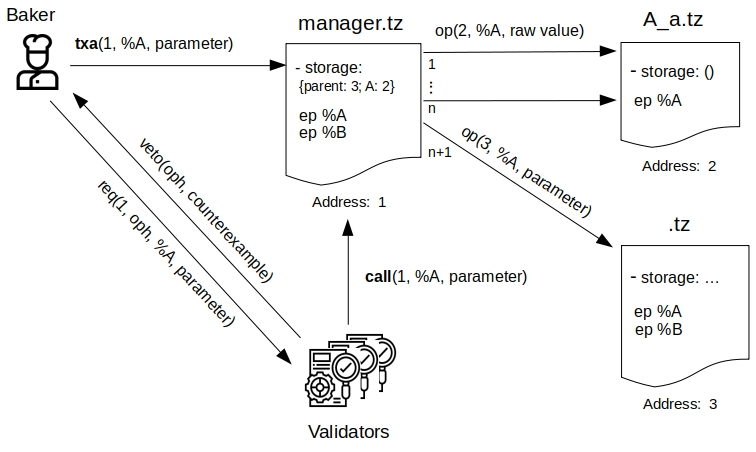
\includegraphics[width=0.9\textwidth]{figures/4-offline_tezos/interaction_modular.jpg}
	\caption{Interaction with a modular contract}
	\label{fig:interaction_modular}
\end{figure}

\subsubsection{Evaluation of the modular approach}
This approach fixes the two central problems of the monolithic approach: by mirroring the interface of the parent contract, the parameters passed to the manager contract can be forwarded directly to the parent contract, regardless of whether the default or an explicit entrypoint was called. As sum type parameters are stripped to the raw values inside the code block (ref. \lstref{lst:mono}), they can be passed to the assertion contract without further ado. Furthermore, the parent contract does not need to be modified, which leads to a much simpler compilation process and allows to extend already originated contracts with assertions. Due to its modularity, adaptions to either contract do not entail the recompilation and origination of all components. The manager is the only component with tight coupling, thus adaptions regarding the manager do not affect any other component. Adaptions to single assertions or the parent affect themselves plus the manager. In order to optimize this and break the tight coupling, one could be inclined to add a setter entrypoint to the manager (as a sort of dependency injection). This, however, would break the mirroring of the parent contract and is thus not possible without annulling one of the key strengths of the design.\\
The approach essentially has to weaknesses: on the one hand, the assertion and the parent cannot be called separately, as they are linked together by the manager. As a result, both the baker and validators execute the assertion, as well as the parent contract, which increases the cost of the contract execution. On the other hand, it exposes a security vulnerability, given that assertions can be bypassed by calling the parent contract directly with unevaluated parameters. This iteration of the design 
does not demand to close this vulnerability, hence possible solutions are not discussed in this thesis.

\section{Backend of the pipeline}
The Tezos backend of the pipeline comprises of the three stages semantic check, type check and compilation. During the semantic check, the common AST is cast to a Tezos-specific AST type. If the assertion contains any data types or operations not supported in Michelson, the assertion contract is rejected. Since the subsequent stages are less straight forward, they are explained in more detail in the following.
\begin{figure}[h]
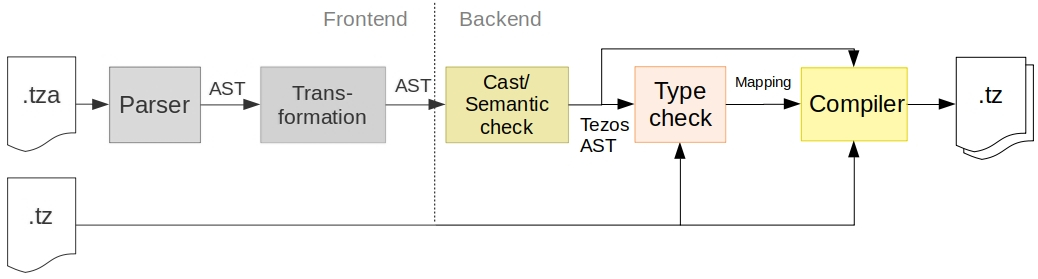
\includegraphics[width=\linewidth]{figures/4-offline_tezos/pipeline_backend}
\caption{The stages of Tezos-specific backend of the compilation pipeline}
\label{fig:pipeline_backend}
\end{figure}

\subsection{Type check}
The task of the type checker is to map the assertions from the given file to the respective entrypoints of the parent contract. To this end, the parameter types have to be compared and matched against each other in order to find a correct assignment. The type checker either reads the code of the parent contract from a given file or retrieves the code from a given address on the blockchain. It must be ensured that the created mapping is injective and unambiguous, i.e., each assertion matches exactly one entrypoint and no entrypoint is covered by more than one assertion.\\
As explained in \secref{sec:tezos}, entrypoints can be selected by calling the default entrypoint and wrapping the parameter into the respective union constructors. Alternatively, they can be called explicitly using their tag and passing the parameter as raw value. The same applies for the assertions - by omitting the tag, the parameter type must be declared in respect to the default entrypoint type. If the assertion states an explicit tag, it may declare the raw parameter type. The tags do not necessarily have to be identical with the tags of the parent contract; in some cases, they may be chosen differently for documentation or for readability purposes. However, the tags can and should be used to resolve ambiguity in the mapping between assertions and entrypoints, that is if several entrypoints share the same input type. Ambiguity can also be caused by the fact that entrypoints can be sub-entrypoints of others, thus assertions overlap if a separate assertion is declared for both super- and sub-entrypoint. This is resolved by detecting overlapping assertions during the type check and rejecting assertion contracts where appropriate. \\
As an exemplification, consider a Michelson contract with five entrypoints (including the \texttt{\%default}):
\begin{lstlisting}[numbers=none, language=Michelson]
parameter (or (int %A) (or %BC (int %B) (int %C)))
\end{lstlisting}
The following assertion contract for the given PC contains some valid and some invalid assertions:
\begin{lstlisting}[language=Assertion]
(assertion %A (i : int) ...)             (* valid *)
(assertion %D (i : int) ...)             (* invalid *)
(assertion (right (left (i : int)) ...)  (* valid *)
(assertion %BC (x : (or int int)) ...)   (* invalid *)
\end{lstlisting}
Due to its tag, the fist assertion can be assigned unambiguously to entrypoint A, whereas for the second it is not apparent whether it should be assigned to entrypoint B or C. Since the tag is omitted in the third assertion, the parameter type is given in respect to the default entrypoint and is assigned to B. The last assertion is invalid because it is overlapping with the previous assertion, which was already assigned to entrypoint B.

\subsection{Compiler}
The transformed and type checked assertion AST needs to be retargeted to Michelson code according to the orchestration scheme. Since the modular approach is less complex to implement and avoids having to decompile the parent code, this section describes a compiler that assembles the assertion and contract code according to \figref{fig:modular_assembly}. The target language of the compiler of the pipeline can either be Michelson directly, or another high-level language which supports Michelson as a target. \secref{sec:tezos} lists some examples of such languages. The chosen language then serves as an intermediate representation (IR) of the assertion and manager code, which is ultimately compiled to Michelson by the compiler of the language. After specifying the steps of the compilation in a general way, the compilation approaches are described and discussed in more detail in \secref{sec:direct} and \ref{sec:IR}.

\subsubsection{Compilation of the assertion contracts}
Since the assertions are independent of each other and the manager code, each of them can be compiled in isolation to a separate Michelson program. The generated code of the assertion body and the parameter type can be plugged into a template that already contains the necessary boilerplate code for a contract.

\subsubsection{Compilation of the manager contract}
Given that the manager contract mirrors the parent contract and assuming that the proposal for the storage type from \lstref{lst:manager_modular} is adopted, the type declarations can be translated directly to the target language. Algorithm \ref{alg:compile_manager} shows the outline of a simplified algorithm that builds the code body recursively. For simplicity, entrypoints that take a sum type as parameter (e.g. \texttt{(or \%AB int int)} are not considered in the algorithm. However, in the actual compiler implementation they need to be taken care of. 
\begin{algorithm}
\caption{Simplified recursive algorithm for building the manager contract}\label{alg:compile_manager}
	\begin{algorithmic}[0]
	\State global storage = \{0: <parent>\} \Comment{Stores the mapping of ids to entrypoints}
	\State global i = 1 \Comment{Counter generating unique ids}
	\Function{compile}{parent parameter type}
	\If{ty = Or(l,r)}
	\State code\_left = compile(l)
	\State code\_right = compile(r)
	\State \Return code\_left + code\_right
	\Else
	\If{assertion exists for this entrypoint}
	\State code = generate\_loop(ty, i)
	\State storage.add(i++, entrypoint tag)
	\Else
	\State code = generate\_forward(ty)
	\EndIf
	\State \Return code
	\EndIf
	\EndFunction
	\end{algorithmic}
\end{algorithm}

The function \texttt{generate\_loop} generates code that does the following:
\begin{enumerate}
\item Retrieve the assertion contract and parent contract addresses from storage
\item Calculate $t$
\item Build a list of $t$ internal operations that call the assertion contract
\item Return the list of emitted operations and the unchanged storage
\end{enumerate}
By passing the next id $i$ to the function, the access to the storage can be hard-wired into the generated code. The address of the parent contract is assumed to always be stored with the id 0. \secref{sec:prob_threshold} stated a formula for calculating $t_{total}$ with the parameters $n$, the size of the search space, and the probability threshold $c$. While $n$ can be calculated from the ranges of the random generator(s), $c$ must be given as parameter to the compiler through the CLI. After $t_{total}$ has been computed, the upper bound of the loop is calculated according to \eqref{eq:t_validator}. 
\begin{equation}\label{eq:t_validator}
t = \lceil t_{total} / \#validators \rceil
\end{equation}

\texttt{generate\_forward} can be generated from a simple template with the id as the only variant and only consists of  an access to the storage and the emission of an internal operation.

\subsubsection{Output}
Besides the target code for the manager and assertion contracts, the compiler should return a piece of template code for the correct storage initialization of the manager. Since this code is passed to the origination operation, it must be in Michelson regardless of the compilation target language. The placeholders or accompanying info should be descriptive enough, s.t. the user can plug in the corresponding addresses after the origination of the parent and assertion contracts. For the example manager contract given in \secref{sec:modular}, the corresponding text output could be\\
\texttt{(Elt 0 <addr parent>; Elt 1 <addr A\_a>; Elt 2 <addr B\_a>)}.

\subsubsection{Direct compilation}\label{sec:direct}
With the direct approach, the compiler generates Michelson code and hence code for a stack machine. Based on the simplicity of stack machines and the assumption that it does not need to generate optimal code, the compiler is expected to be simple \cite{cs5641}\cite{ferr_compiler}\cite{wiki:stack_machine}. As already indicate in the general part, the resulting contracts contain repeating structures and patterns for each input, which can be exploited by using template code during compilation. After compilation, the Michelson programs can be sanity-checked by type checking them using the provided Tezos libraries.

\paragraph{Assertion contracts}
\lstref{lst:contract_templ} shows a possible template for an assertion contract --- the placeholder \texttt{<?>} marks the locations where the individual code is inserted. Lines 3-5 prepare the stack, s.t. the parameter and storage are the two top elements. The lines below the placeholder for the body clean up the stack and leave it according to calling convention, i.e., the program returns an empty list of internal operations and the unit storage.
\lstinputlisting[label=lst:contract_templ, language=Michelson, caption=Template code for assertion contracts in Michelson, numbers=left]{listings/assertion_template.tz}

\paragraph{Manager contract}
The generation of the \texttt{parameter} and \texttt{storage} primitives is trivial --- the parameter type can be carried over directly from the parent contract, whereas the storage type is a constant (\texttt{(map int address)}). Based on the algorithm given previously, the code body is generated by nesting \texttt{IF\_LEFT} instructions recursively (cf. \lstref{lst:entrypoints}). The adapted algorithm is given in Algorithm \ref{alg:compile_manager_direct}.
\begin{algorithm}
\caption{Modification of algorithm \ref{alg:compile_manager} for direct compilation}\label{alg:compile_manager_direct}
	\begin{algorithmic}[0]
	\State ...
	\Function{compile}{parent parameter type}
	\If{ty = Or(l,r)} \Comment{Compile sum types to a branching}
	\State code\_left = "IF\_LEFT {" + compile(l) + "}"
	\State code\_right = "{" + compile(r) + "}"
	\State \Return code\_left + code\_right
	\EndIf
	\State ...
	\EndFunction
	\end{algorithmic}
\end{algorithm}

Owing to Michelson being a low-level language, the templates for the functions \texttt{generate\_loop} and \texttt{generate\_forward} go beyond the scope of this subsection. In order to provide an idea of how the generated code could look like, appendix \ref{apx:manager_michelson} contains two example contracts, one of which contains manager code for a non-empty and the other one for an empty assertion. The code was generated by the Liquidity compiler from two contracts written in Liquidity, as this provides a more compact and readable representation of the program logic. The corresponding source code can be found in \secref{sec:IR}.

\paragraph{Evaluation}
Compiling to Michelson directly is beneficial due of several reasons --- the pipeline stays streamlined and outputs the final contracts ready for origination. It does not introduce dependencies to external tools and their support for new protocol versions of Tezos. Besides, the new instructions only have to be added to Tezos' protocol code, whereas using external tools and languages would need to be patched as well in order to support them. \\
When it comes to verifying the compiler and integration testing of the pipeline, however, the low-level output causes more complexity than a high-level output. Due to the extend and restricted readability of non-trivial Michelson programs, their correctness is not always apparent in an instant. Tests can, on the one hand, compare the output with verified target contracts for a range of inputs, which requires a lot of Michelson code written by hand for each input. They, in turn, can also be prone to errors. On the other hand, the generated contracts can be tested as a black box using the test frameworks provided by Tezos, which use sandboxed networks to interact with contracts-under-test.

\subsubsection{Compiling to an IR}\label{sec:IR}
Instead of generating Michelson code directly, the compiler could also generate code in one of the high-level languages that provide a compiler with Michelson as a target. The output of the pipeline is then passed to this compiler in order to retrieve the final contracts. If the toolchain of the intermediate language doesn't provide a programmatic interface, the pipeline thus has to be extended with a separate step of procedure, as shown in \figref{fig:pipeline_liq}. This section demonstrates the implementation of this approach on the basis of Liquidity, hence the corresponding file extension \texttt{.liq}.
\begin{figure}[h]
\centering
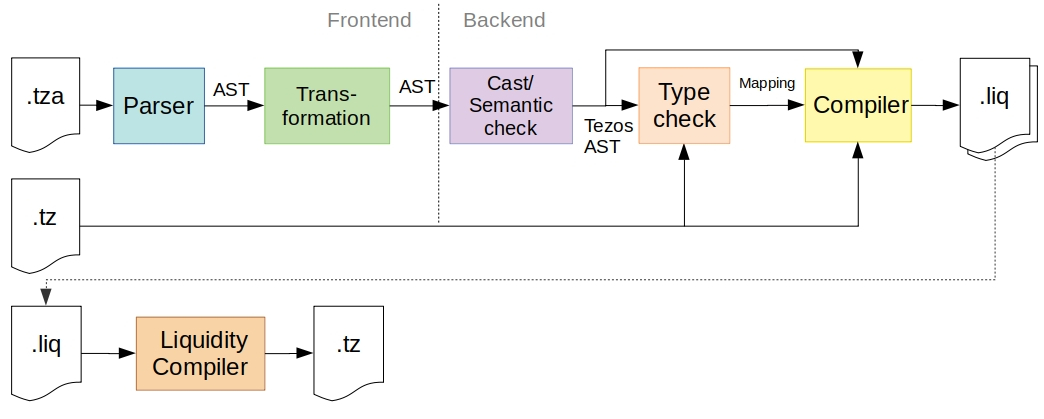
\includegraphics[width=\linewidth]{figures/4-offline_tezos/pipeline_liq}
\caption{Pipeline with IR compilation and an external toolchain}
\label{fig:pipeline_liq}
\end{figure}

\paragraph{Assertion contracts}
\lstref{lst:contract_templ_liq} shows the equivalent of the assertion contract template given in \lstref{lst:contract_templ}. Since the Liquidity compiler takes care of the handling of the stack, it basically consists only of a storage type declaration, a function signature and the ``empty'' return type.
\lstinputlisting[label=lst:contract_templ_liq, language=Michelson, caption=Template code for assertion contracts in Liquidity, numbers=left]{listings/assertion_template.liq}

\paragraph{Manager contract}
Liquidity contracts are a list of OCaml-like functions that take a parameter and a storage. Instead of declaring the contract parameter type globally and nesting the code for each entrypoint, each entrypoint thus is declared as a separate function with a local parameter type. During compilation, the contract parameter type will then be composed according to the order of functions. 
Due to Algorithm \ref{alg:compile_manager} being left recursive, the output will automatically retain the correct order of entrypoints. In fact, the only adaptions necessary are the output of the two functions \texttt{generate\_loop} and \texttt{generate\_forward}, which should not only generate the code body, but return a coherent function. The function \texttt{entrypointA} in \lstref{lst:manager_templ_liq} is an example of such a function for an empty assertion. The non-empty version of the manager code can be found in appendix \ref{apx:apx:manager_liq}. As already noted, extracting a pure template for the code exceeds the scope of this section.
\lstinputlisting[label=lst:manager_templ_liq, language=Michelson, caption=Manager code in Liquidity for an entrypoint with an empty assertion, numbers=left]{listings/manager_forward.liq}

\paragraph{Evaluation}
This approach takes advantage of the usually more sophisticated high-level language compiler; they may provide options for optimizing generated code and are already thoroughly tested \cite{liq_repo}\cite{ligo_repo}. In contract to low-level code, the output of the pipeline compiler is easier to be verified, as it can be read like, for instance, an OCaml program. Providing target contracts for integration tests can be done much more efficiently and more reliable. \\
Besides the amenities of these compilers, this approach has a crucial disadvantage of introducing an external dependency. The compiler of the respective language has to be extended with the additional Michelson instructions as well, requiring a fork of the project. Furthermore one has to rely on continuous support of new protocol versions in the root project and integrate the updates into the own codebase. All things considered, the effort for extending both Michelson and the compiler of the IR, followed by a continuous effort of version management, may outweigh the benefits of this approach.

When returning to the orchestration approach of generating a monolithic contract, using Liquidity as an IR would allow to decompile the parent contract using the decompiler of its toolchain. Since the Liquidity compiler handles the composition of the contract parameter type and the code nesting, the assertion function simply have to be appended to the parent code, which significantly decreases the compilation complexity.

\section{Cost analysis}\label{sec:cost_analysis_distributed}
What remains to be evaluated is the cost of checking a formula with the proposed approach, and how they relate to the costs for a local validation which were analysed in \secref{sec:usecase_cost}. The previous analysis defined \eqref{eq:gas_transaction} to calculate the gas consumption of a transaction, including the emitted operations. For each validator, the transaction calling the manager contract emits $t+1$ internal operations, whose gas consumptions are also dependent of the input parameter. Based on the $t+1$ additional base, as well as deserialization and parsing costs of the parameter alone, it can be concluded that the total gas consumption of $n$ total distributed test runs is higher than the cost of checking $n$ values locally. \\
The differential can be measured by implementing the orchestration scheme for the two dummy contracts given in \secref{sec:usecase_cost}. Appendix \ref{apx} contains the code of all three components for each of them. In order to measure the gas consumption for a comparable amount of executions as during the initial cost analysis, the probability threshold $c$ is set to $\frac{1}{e}$, s.t. that the necessary number of total test runs is $n$. However, it needs to be pointed out, that the actual number of test runs executed can only be a multiple of the number of validators (cf. \eqref{eq:t_validator}). \figref{fig:cost_distributed} shows the reported gas consumption per validator, i.e., a $32^{th}$ of the total cost for checking an assertion for the given threshold. Due to \eqref{eq:t_validator}, the cost function approximates a step function.
\begin{figure}[t]
\centering
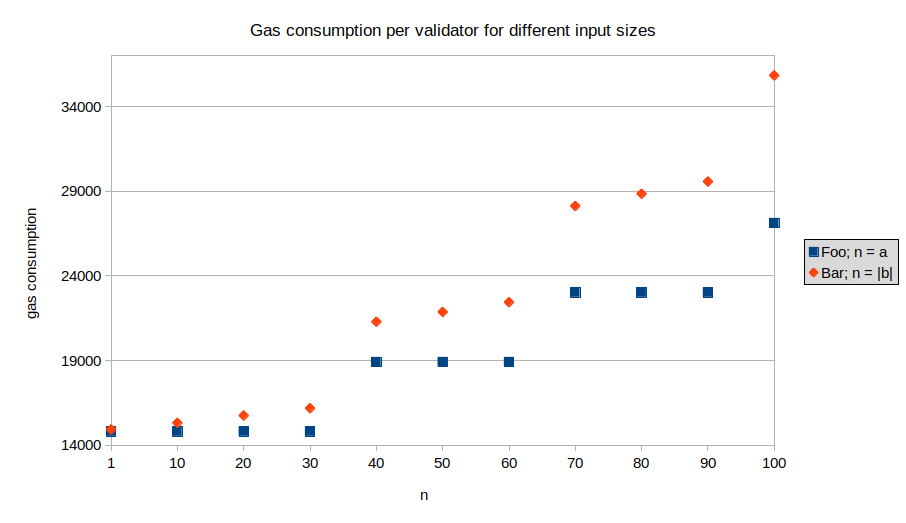
\includegraphics[width=0.9\linewidth]{figures/4-offline_tezos/cost_analysis}
\caption{Gas consumption per validator of transactions calling \texttt{Foo} and \texttt{Bar} for increasing input sizes}
\label{fig:cost_distributed}
\end{figure}
The results show that the cost incurred by a single validator checking $t$ values is already considerably higher than by checking the property locally. Moreover, the cost-performance ratio is even worse, as the confidence that the property is indeed satisfied is only around 63\% with the given parameters. In conclusion to these results, it may be worth looking into some alternative approaches. \secref{sec:alt_random} already mentions the possibility to coordinate the validators for a systematic iteration of the search space. Alternatively, the proposed orchestration could be modified, s.t. the manager and assertion code are not implemented as separate contracts, but with one single contract. Instead of $(t+1)$ internal operations, one only has to pay for one internal operation that calls the parent contract, hence avoiding the base, deserialization and parsing costs for each test run. Similar to the monolithic orchestration approach, this increases the complexity of the compilation process.\\ Another idea worth exploring is the adaption of the blockchain protocol to avoid user costs for assertion checking, similar to the regular validation of blocks \cite{tezos_docs}. Instead of being paid by the user in gas, validators could be given a reward for checking an assertion, or a particularly high one for finding a counterexample. 

\todo{Cheaper for the network if not all validators have to execute the whole local check! however, placing these costs on the users will cause them to use the local approach -> users need incentives to use it too! -> blockchain protocol could/should solve this! (e.g. use rewards instead of costs)}
\todo{Every transaction is processed at every node in the network,which limits throughput}


\section{Representing counterexamples}
There still remains an open question concerning the proposed implementation that could be answered in detail within the scope of this thesis - the representation and validation of a counterexamples. The interaction scheme in \figref{fig:interaction_modular} suggests, that validators publish an instance of a counterexample to the network if they found one. However, it has yet to be specified how the counterexample is represented and double-checked by the other validators. With the \texttt{failwith} instruction, the top element of the stack can be exposed \cite{tezos_docs}, providing a way to return an interpretable expression from the interpretation context \cite{tezos_repo}. Thus, as a first approximation, the counterexample could be represented as a tuple of assertion code and a list of randomly generated values. For instance, the counterexample for the assumption ``p is a prime'' (cf. \eqref{eq:prime}) is represented by \\
\texttt{(n >= 2 \&\& n <= sqrt(p) \&\& p\%n = 0, <random value for n>)}. \\
For validation of the counterexample, this tuple, together with the respective operation hash of the initial transaction this counterexample refers to, is published to the network. The other validators then interpret the given code with the respective value(s) and either confirm or object the counterexample. As Tezos transmits data as byte sequences, the counterexample needs to be unparsed and serialized, or deserialized and parsed respectively. If the cost for checking assertions is paid for be the user (in form of gas), then these costs have to be added to the total costs as well.\\
In order to prevent denial-of-service attacks by spamming the network with false counterexamples, the protocol should implement penalties for such cases. Details about this and possible rewards for valid counterexamples should be considered in the protocol design.